%Préambule du document :
\documentclass[12pt, a4paper]{book}
%\usepackage[latin1]{inputenc} 
\usepackage[utf8]{inputenc} % accents
\usepackage{gensymb} % degree symbol ° (\degree)
\usepackage[T1]{fontenc} % | "`pipe"' character
\usepackage{graphicx}
\usepackage{titling}
\usepackage{amssymb} 
\usepackage{minitoc} % chapter's tocs
\usepackage{authblk} % author affiliations
\usepackage{fancyhdr} % modify the headers
\usepackage{tabularx} % tables not larger than A4
\usepackage[table]{xcolor} %colors inside the tables
\usepackage{float}
\usepackage{multicol} % multiple columns in some sections
\usepackage[inner=2cm,outer=2cm]{geometry} %A4 margins
\usepackage{siunitx}
\usepackage[labelfont=bf, margin=0.5cm]{caption} % for figure captions in minipages
\usepackage{hyperref} %link references (toc, citations) inside document
\usepackage{natbib} % to cite with parentheses and plain text et only year if you please...
\usepackage{amsmath}
 \usepackage{fixltx2e} % allows overrightarrow to be in caption
 \MakeRobust{\overrightarrow}




\bibliographystyle{plainnat} % reference style
\renewcommand{\bibname}{References} %Rename "`bibliography"' => "`references"'

\hypersetup{
    colorlinks,
    citecolor=brown,
    filecolor=green,
    linkcolor=red,
    urlcolor=blue
}
\hypersetup{linktocpage}


\pagestyle{fancy}
\fancyhead{}
\fancyfoot{}
\fancyhead[RO,LE]{\thepage}
\fancyhead[LO]{\leftmark}
\fancyhead[RE]{\rightmark}
\setcounter{tocdepth}{1} % we only want chapters and sections in toc
\setcounter{minitocdepth}{2} %we want sections and subsections in chapters' minitocs

\pretitle{%
  \begin{center}
  
  
\includegraphics[width=17cm]{../Logo_software.png}\\[\bigskipamount]
}
\posttitle{
\\
  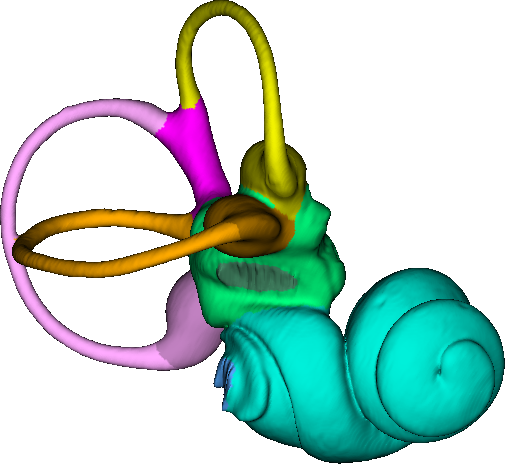
\includegraphics[width=8cm]{tutorial05.png}\\[\bigskipamount]
\end{center}}

%\postdate{
%
\includegraphics[width=15cm]{logo_affiliations.png}
%}

\title{Tutorial 05: working with flags}



%\titlepicture[width=13cm]{Logo_software.png}
\author{Renaud LEBRUN}
\affil{Institut des Sciences de l'Evolution, Université de Montpellier, France}
\date{\today} 

\def\chaptername{Tutorial}
\setcounter{chapter}{5}
%Corps du document :
\begin{document}

	\dominitoc

\maketitle


\faketableofcontents

%\chapter{Working with landmarks}
\addstarredchapter{Working with flags}

\markboth{Tutorial 05: Working with flags}{}

\minitoc 
Tutorial 04 includes:
\begin{itemize}
\item One .ntw (MorphoDig project) file
\item One .vtk surface file representing a right inner ear of \textit{Mus musculus}
\item One .pos (position) file 
\item One .ori (orientation helper labels) file 
\item The present .pdf document
\end{itemize}





\section{About the specimen}

%\addcontentsline{toc}{section}{About the specimen}
The surface file enclosed in this tutorial represent three-dimensional reconstruction of the right inner ear of a house mouse (\textit{Mus musculus}) obtained by computerized microtomography at the MRI \si{\micro} CT platform housed at the ISEM.\\
Before using this tutorial, please download and read MorphoDig User Guide.


\section{A brief overview of enclosed files}
		Download and unzip the files associated to this tutorial. Open MorphoDig.
\subsection{Mouse inner ear surface and position files}
	You may open the enclosed .vtk surface file (File -> Surface -> Open Surface, then select "Mouse\_right\_ear.vtk", or drag and drop this file in the 3D main window). When opened
this way, the corresponding opened surface object is drawn grey, which indicates that this surface
is selected. You may interact with selected objects in different ways (see MorphoDig user guide for
further explanations).\\


By default (\includegraphics[scale=0.7]{../images/06/camera/move_cam2.png}), the camera rotates around the center of mass of all opened objects. This behavior is useful when the center of mass of an object (or of several ones) is far from the origin of the coordinate system. But by pressing the camera button (\includegraphics[scale=0.7]{../images/06/camera/move_cam2.png} -> 
\includegraphics[scale=0.7]{../images/06/camera/move_cam.png}), the camera will revolve around the center of the coordinate system (x=0, y=0, z=0).  The display grid is drawn using different colors depending on the camera rotation center (see Fig. \ref{grid_color} p.\pageref{grid_color}).



 As a general rule, when opening a new surface, it is strongly advised to change its position in order that it matches the 6 predefined camera positions :\\

\includegraphics[scale=0.7]{../images/06/camera/camera_right.png} view object from right side \\

\includegraphics[scale=0.7]{../images/06/camera/camera_left.png} view object from left side\\

\includegraphics[scale=0.7]{../images/06/camera/camera_front.png} view object from front side (default camera position)\\

\includegraphics[scale=0.7]{../images/06/camera/camera_back.png} view object from back side\\

\includegraphics[scale=0.7]{../images/06/camera/camera_above.png} view object from above\\

\includegraphics[scale=0.7]{../images/06/camera/camera_below.png} view object from below\\

In "object interaction mode(
\includegraphics[scale=0.7]{../images/04/move_mode.png})", selected objects can be translated and rotated using the mouse left and middle buttons (in landmark 
\includegraphics[scale=0.7]{../images/04/Landmarks2.png} and camera  
\includegraphics[scale=0.7]{../images/04/camera_mode.png} selection modes, you also need to maintain ``CTRL" button pressed while dragging the left mouse button to achieve rotation and translation of selected objects). Alternatively, you may also use the "yellow sliders" located on the right side of the 3D main window to accomplish rotation and translation of selected objects. Rotation is achieved around the global center of mass of all currently selected objects.\\
\begin{figure}
  \centering
  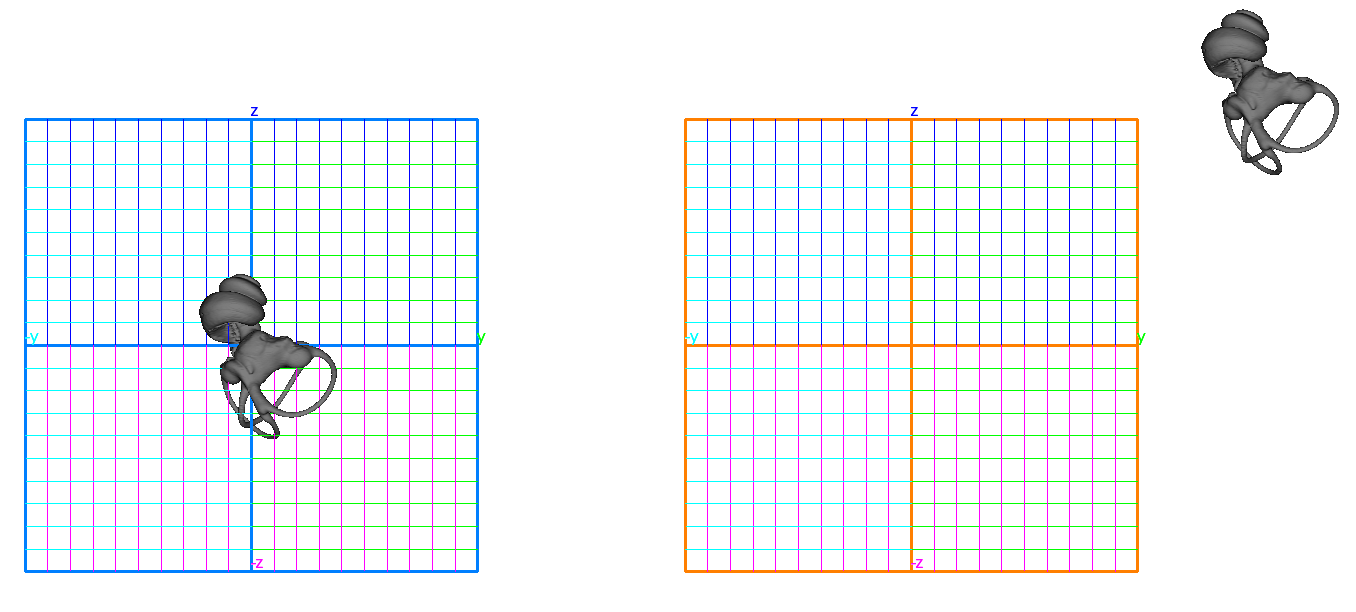
\includegraphics[scale=0.3]{grid.png} 
	\caption{Grid display color.  Left: when the camera revolves around the center of mass of all opened objects, the grid has a blue outline. Right: when the camera revolves around the origin of the coordinate system (x=0, y=0, z=0), the grid outline is displayed in orange.}
\label{grid_color}
 
\end{figure}

A convenient way to orient a right inner ear in a biologically relevant way is done as follows (see Fig. \ref{orientation} p.\pageref{orientation}):\\
1) place camera to view object from the front side (
\includegraphics[scale=0.7]{../images/06/camera/camera_front.png})\\
2) place the lateral semi-circular canal in the horizontal plane (x-y plane)\\
3) place camera  to view object from above ( 
\includegraphics[scale=0.7]{../images/06/camera/camera_above.png} )\\
4) rotate the inner around the z axis ("rz" yellow slider) until the later semicircular points towards the top left-hand part of the screen, and the cochlea points towards the bottom right-hand of the screen.\\
That way, when viewing the inner ear from the front side (
\includegraphics[scale=0.7]{../images/06/camera/camera_front.png}), it is approximately oriented in the same way as it would be within the cranium viewed from the front side as well.\\

The present tutorial contains a .pos (position) file, which you may open in order to place correctly the right ear of the house
mouse (File -> Position-> Open Position for selected surfaces, then choose "Mouse\_right\_ear.pos", see Fig. \ref{orientation} p.\pageref{orientation}). As we plan to place curve node landmarks and curve handle landmarks inside the cochlea and the semicircular canals, please select the right inner ear surface (CTRL+A, or drag right mouse button to draw a selection rectangle) and change its transparency (Edit Selected Surface->rendering modifications->Change transparency -> then give a value smaller than 100).\\
All opened surfaces can be unselected by pressing "CTRL +D", or selected by pressing "CTRL +A". All selected objects can be deleted by pressing "Del".

\begin{figure}
  \centering
  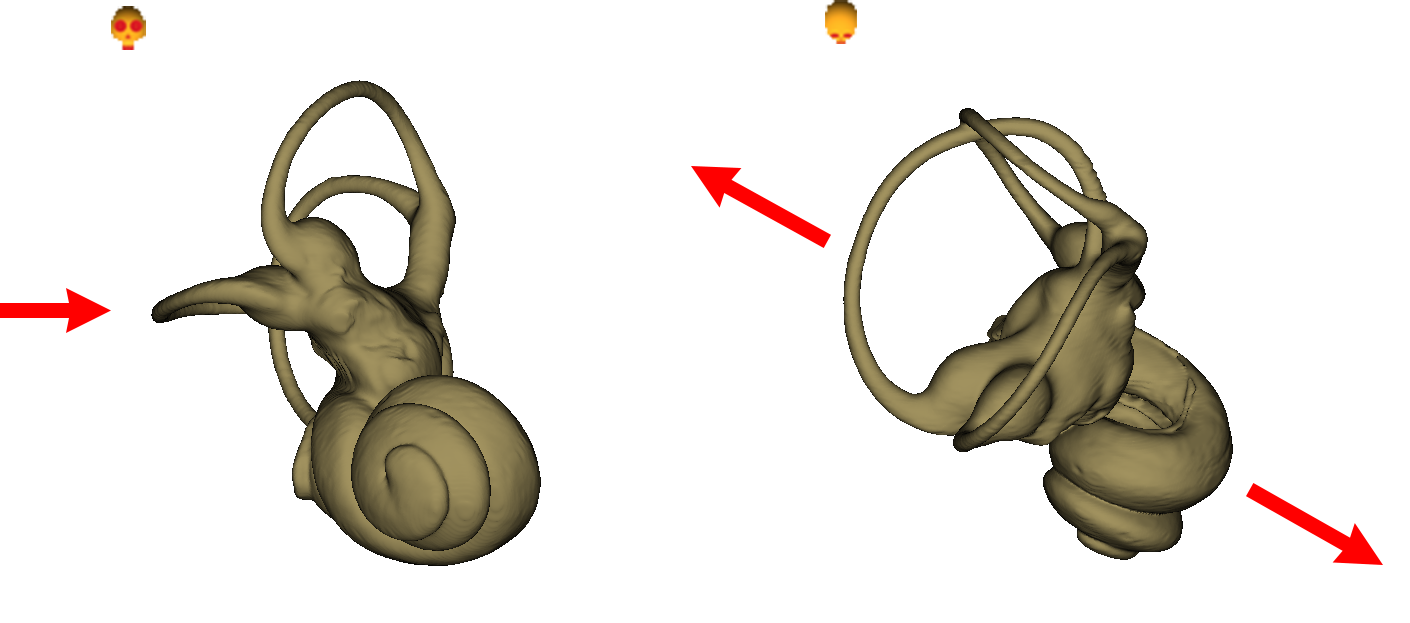
\includegraphics[scale=0.3]{pos.png} 
	\caption{A convenient way to orientate right inner ears.  Left: when viewed from the front side, the lateral canal is placed horizontally. Right: when viewed from above, the cochlea points towards the bottom right-hand of the screen, and the lateral canal towards the top left-hand of the screen.}
\label{orientation}
 
\end{figure}

\subsection{Mouse inner ear project file}
The present tutorial contains a project .ntw file, which may be useful to directly open the right inner ear
 in a convenient position, to make it transparent and to give it a color. First, delete all currently opened objects
(press "CTRL+A", then press "Del"). Then open the enclosed .ntw file (File -> Open Project, then select
"Mouse\_right\_ear.ntw"). Once loaded, the right inner ear surface is opened, is given the position
enclosed in the "Mouse\_right\_ear.pos" file, a color and a transparency. Note that the newly opened
surface is unselected.\\


\subsection{Mouse inner ear flag file}
Prerequisite : make sure that the mouse right inner ear surface is loaded, and that it is correctly positioned. 
You can load the enclosed .flg file (File->Flags->Open Flags-> Mouse\_right\_ear.flg or drag and drop this file directly in the 3D main window), which contains 13 flags.   


\subsection{Mouse inner ear .ori file}
The present tutorial contains a .ori file, which contains orientation labels for the coordinate system
orientation helper. You can load this file the enclosed .ori file ("File->Orientation helper labels -> Open Orientation labels", then select
"Mouse\_cranium.ori"). Once loaded, the system coordinate orientation helper will show the following
labels :\\
+z axis : superior\\
-z axis : inferior\\
+y axis : medial\\
-y axis : lateral\\
+x axis : proximal\\
-x axis : distal\\
You may set your own orientation axis labels with the “Edit orientation labels” window (Edit-> Edit orientation labels)

\section{Flag digitization with MorphoDig}


\subsection{Flag rendering options}
Flags are rendered in MorphoDig the following way: a sphere is placed at the location of interest and rendered; additionally, a thin cylinder of a defined length is drawn between this location and the place where the label is rendered. 
conventional landmark location (do not try to select / unselect the label or the line directly, this will
have no effect).
You can change the way flags are rendered in the "Landmark and flag options" window
(Edit->Edit landmark and flag rendering options, Fig. \ref{flag_rendering_options} p.\pageref{flag_rendering_options}). You can choose the default flag length and the default flag color. As the structure we investigate in this tutorial is quite small (around 4 mm long), I recommend you to set the flag length to about 0.5mm.


\begin{figure}
  \centering
  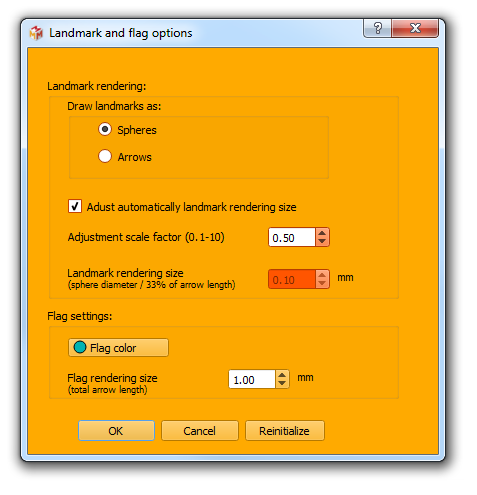
\includegraphics[scale=0.55]{../images/08/landmark_flag_options.png} 
	\caption{Landmark and flag options window.}
\label{flag_rendering_options}
\end{figure}

\subsection{Creating new flags}

Press “
\includegraphics[scale=0.7]{../images/04/flag_landmarks.png}” to activate flag digitization mode (this mode is \textbf{NOT} active by default)

\subsection{Interacting with flags}
When digitizing flag landmarks, I recommend to press "
\includegraphics[scale=0.7]{../images/04/Landmarks2.png}" to activate the "Landmark mode". When active,
only landmarks (among which flag landmarks) can be selected/unselected via right mouse button drag/click. Flag landmarks can be set
on surfaces by pressing "L" + left mouse click.
 If a single flag landmark is selected, its position can be moved
on another part of the surface by pressing "L" + right mouse click (nothing happens if no flag
is selected or if more than one flag are selected). Also, you may need to move flags away
from the object’s surface (for instance when you want to place a flag at the center of a foramen):
once selected, the position of a given flag can be moved by using the usual mouse (CTRL + middle click + mouse drag) and GUI controls.\\


\begin{figure}
  \centering
  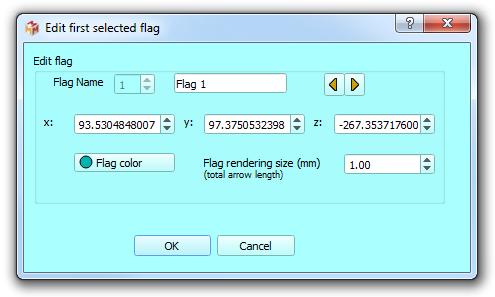
\includegraphics[scale=0.55]{../images/06/objects/edit_flag.png} 
	\caption{Edit first selected flag window.}
\label{first_flag_edit}
\end{figure}


Flag landmark selection / unselection is performed as for other 3D objects:\\
- \textbf{Selecting flags 1 by 1}: press "CTRL +D" to unselect all 3D objects and click on "
\includegraphics[scale=0.7]{../images/06/objects/flag_edit.png}": this button opens the "Edit first selected flag" window (see Fig. \ref{first_flag_edit} p.\pageref{first_flag_edit}). Then click on 
\includegraphics[scale=0.7]{../images/06/objects/s_right.png} and 
\includegraphics[scale=0.7]{../images/06/objects/s_left.png} to navigate through all existing flags and to select them 1 by 1. That way, you can edit the properties of each of them individually.\\
- \textbf{Selecting flags with the mouse}: maintaining the right mouse button pressed while dragging the mouse will draw a selection rectangle. Once the right mouse button has been released, all unselected flags laying underneath the selection rectangle will be selected (and all selected surfaces will be unselected).\\
- \textbf{Selecting all flags (and all other 3D objects)}:\\all opened flags (+ all other objects) can by selected by pressing "CTRL +A" (conversely, all flags (+ all other objects) can be unselected by pressing "CTRL +D")\\




\subsection{Saving flags}
To save all digitized landmarks, go in "File->Flags->Save Flags".

\subsection{Saving the project}
Saving a "project" makes it possible to save all opened selected objects (surface of the inner ear and its position+color, flags) altogether instead of one by one. 
To save all opened objects, do the following sequence of actions:\\
1) press "CTRL + A" to select all objects\\
2) click on "File->Project->Save Project" or on the button "save project" (
\includegraphics[scale=0.03]{../images/03/save_data.png})  inside the main window.\\
3) choose the desired options in the "Save Project" window (see Fig. \ref{save_project_file} p.\pageref{save_project_file} and the User Guide for further details regarding the available options)
\begin{figure}
  \centering  
 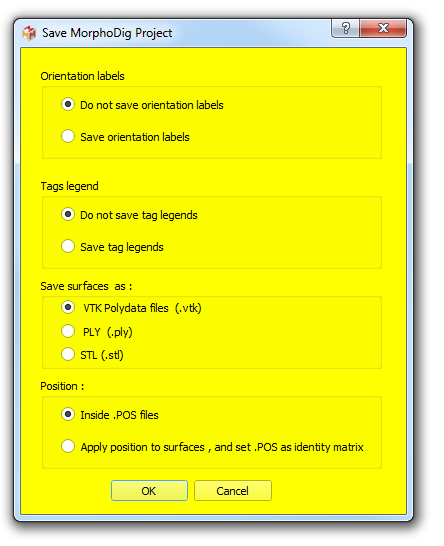
\includegraphics[scale=0.5]{../images/07/project/save_ntw.png}
 \captionof{figure}{Save project window.}
\label{save_project_file}
\end{figure}

The advantage of working with projects is that all involved objects (surfaces, flags, positions and colors) can be reloaded later all at once (and not 1 by 1). 

\section{Acknowledgements}
Thanks to the MRI imaging platform for the access to imaging facilities.

%\nocite{*}   % All bibliography items appear without citation in the text

%\cleardoublepage
%\phantomsection

%\addcontentsline{toc}{chapter}{References}
%  \bibliography{References/UsersGuide}		
\end{document} 

